% The Clever Algorithms Project: http://www.CleverAlgorithms.com
% (c) Copyright 2011 Jason Brownlee. Some Rights Reserved. 
% This work is licensed under a Creative Commons Attribution-Noncommercial-Share Alike 2.5 Australia License.

% Name
% The algorithm name defines the canonical name used to refer to the technique, in addition to common aliases, abbreviations, and acronyms. The name is used in terms of the heading and sub-headings of an algorithm description.
\section{Logistic Regression} 
\label{sec:logistic}
\index{Logistic Regression}
\index{logit}

% other names
% What is the canonical name and common aliases for a technique?
% What are the common abbreviations and acronyms for a technique?
\emph{Logistic Regression, Logit, Logit Model, Logistic Model, Binomial Logistic Regression, Binary Logistic Regression}

% Taxonomy: Lineage and locality
\subsection{Taxonomy}
% To what fields of study does a technique belong?
Logistic Regression is a regression method from the field of statistics, although us better understood as a classification method. It is considered a special case of Generalized Linear Regression (GLR), it is an example of a Generalized Linear Model (GLM) and may be considered an extension of Linear Regression.

% extensions
Ordered Logistic Regression is an extension of Logistic Regression that can handle ordinal dependent variables, and Multinomial Logistic Regression that can handle nominal (categorical) dependent variables. Other common extensions include Stepwise Logistic Regression for variable selection and Regularized Logistic Regression.

% Strategy: Problem solving plan
% The strategy is an abstract description of the computational model. The strategy describes the information processing actions a technique shall take in order to achieve an objective. The strategy provides a logical separation between a computational realization (procedure) and a analogous system (metaphor). A given problem solving strategy may be realized as one of a number specific algorithms or problem solving systems. The strategy description is textual using information processing and algorithmic terminology.
\subsection{Strategy}
% What is the information processing objective of a technique?
Logistic Regression fits data to a logistic (sigmoidal) function and makes predictions of the probability of the occurrence of an event. 
% What is a techniques plan of action?
A logistic function is used because it can take any values (positive or negative) and produce a value between 0 and 1. The logistic function is influenced by a logit function which take a variable derived from a sum of the weighted attributes. The logit function is the natural logarithm of the probability of the dependent variable equalling one.

The regression coefficients (sometimes called `weights') are fit by minimizing the maximum likelihood loss function. A Quasi-Newton method is commonly used to solve the system of linear equations to find stable coefficients.

% Heuristics: Usage guidelines
% The heuristics element describe the commonsense, best practice, and demonstrated rules for applying and configuring a parameterized algorithm. The heuristics relate to the technical details of the techniques procedure and data structures for general classes of application (neither specific implementations not specific problem instances). The heuristics are described textually, such as a series of guidelines in a bullet-point structure.
\subsection{Heuristics}
% What are the suggested configurations for a technique?
% What are the guidelines for the application of a technique to a problem instance?

\begin{itemize}
	\item It is a relatively fast method to create a model and commonly does not require any configuration parameters.
	\item The resulting model is considered understandable and always produces a prediction $\in[0,1]$.	
	\item It does not assume a linear relationship between the independent variables and the dependent variable as with Linear Regression. 
	\item The result is a probability of the occurrence of an event that maybe interpreted as such, and/or in turn be discretized to a binary classification prediction.
	\item Training data with a minimum of 10 events per independent variable is recommended \cite{Peduzzi1996}.
	\item It is of a class of model where on some problems more data can result in a better fit.
	\item The sign of a regression coefficient may be interpreted as the positive or negative contributions of an attribute to the resulting probability, and the magnitude represents the influence of the attribute.
	\item The use of a logistic function means that input attributes can take any value, the bounds do not need to be known prior to building the model.
	\item It can only handle real-valued dependent variables.
	\item Missing values must be handled explicitly or those records removed.
	\item The method requires that the independent variable be related to the logit by a linear relationship.
	\item It does not require normally distributed variables.	
\end{itemize}


% sample script in R
\subsection{Code Listing}
% listing
Listing~\ref{stats_logistic_regression} provides a code listing of the Logistic Regression method in R. Figure~\ref{plot:logistic_regression_result} provides a plot of the training dataset with the line of best fit highlighted.

% algorithm and package
The example uses the \texttt{glm()} function in the \texttt{stats} core package which is responsible for fitting Generalized Linear Model models \cite{RDCT2011a}. The configuration specified a binomial distribution for the response variable with a logit link function. The implementation uses the Iteratively Re-weighted Least Squares (IWLS) method to fit. IWLS is a quasi-Newton optimization method (also called Fisher's Scoring Method) that approximates the Hessian matrix with Fisher's information matrix. For more information on this library type: \texttt{library(help="stats")}, and for more information on the function type: \texttt{?glm}.

% problem
The test problem is a three-dimensional classification problem, where the $x$ and $y$ attributes are numerical and drawn from normal distributions around 0 and 4. A class value of ``a'' or ``b'' is assigned to each coordinate such that the two classes can be separated by a straight line. The dataset is split into a training set to make the model comprised of 67\% of the samples, and a test set for assessing the model comprised of 33\% of the samples.

\lstinputlisting[firstline=7,language=r,caption={Example of Logistic Regression in R using the \texttt{glm} function of the \texttt{stats} core package.}, label=stats_logistic_regression]{../src/algorithms/regression/stats_logistic_regression.R}

\begin{figure}[htp]
\centering
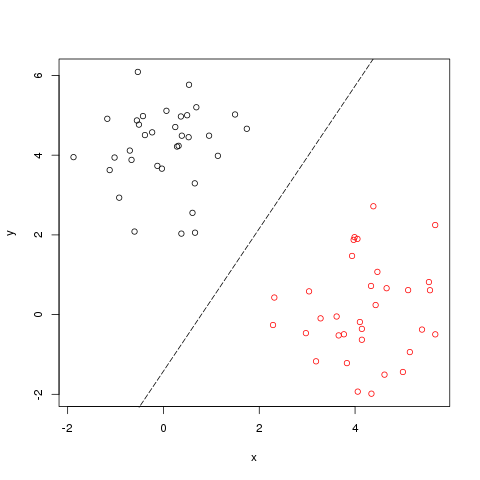
\includegraphics[scale=0.45]{a_regression/logistic_regression_result.png}
\caption{Plot 2D training dataset with the line of best fit.}
\label{plot:logistic_regression_result}
\end{figure}

% other
% glmnet can fit large logistic regression models

% References: Deeper understanding
% The references element description includes a listing of both primary sources of information about the technique as well as useful introductory sources for novices to gain a deeper understanding of the theory and application of the technique. The description consists of hand-selected reference material including books, peer reviewed conference papers, journal articles, and potentially websites. A bullet-pointed structure is suggested.
\subsection{References}
% What are the primary sources for a technique?
% What are the suggested reference sources for learning more about a technique?

% primary sources
\subsubsection{Primary Sources}
% GLMs
The development of Logistic Regression may be traced back to the classic paper that defined Generalized Linear Models (GLMs) by Nelder and Wedderburn \cite{Nelder1972}. In it they describe a regression framework where each model assumes a distribution in the response (such as Normal, Binomial, Possion and Gamma), a linear predictor, and a link function. In the case of a selected Binomial distribution, the link function was selected as probit or logit (generally considered equivalent for these purposes). This combination under the GLM framework became known as Logistic Regression.
% early study
McCullagh and Nelder provide a presentation of GLMs in their seminal text \cite{McCullagh1989}.


% more info
\subsubsection{More Information}
% general references
There are many excellent books dedicated to Logistic Regression, some examples include a text by Pampel that provides a practical introduction to the method \cite{Pampel2000}, a text on applied Logistic Regression by Hosmer and Lemeshow that provides a wealth of references \cite{Hosmer2000}, and book by Kleinbaum, Klein, and Pryor that is also an excellent self-paced introductory text \cite{Kleinbaum2010}.

% data mining and R
Komarek and Moore promote the use of the method in modern data mining, suggesting modifications to the fit procedure to decrease computational complexity \cite{Komarek2005}.



% END
